\documentclass[aps,prl,onecolumn,superscriptaddress,groupedaddress,nofootinbib,floatfix,notitlepage]{revtex4-1}
   
%% Note for comments
%% use two %
%% use a space after %% write here

%% packages
\usepackage{graphicx,psfrag}
\usepackage{mathrsfs}
\usepackage{amsmath,amsfonts,amssymb}
\usepackage{multirow}
\usepackage{comment}
\usepackage[normalem]{ulem}
\usepackage{hyperref}
\usepackage{makecell}

%% macros

\newcommand{\be}{\begin{equation}}
\newcommand{\ee}{\end{equation}}
\newcommand{\bea}{\begin{eqnarray}}
\newcommand{\eea}{\end{eqnarray}}
\newcommand{\bel}{\begin{align}}
\newcommand{\eel}{\end{align}}
\newcommand{\stext}[1]{\text{#1}}
\newcommand{\tento}[1]{\times 10^{#1}}

\def\l{\ell}
\def\lm{\ell m}
\def\p{\partial}
\def\Lie{{\cal L}}
\def\non{\nonumber}                     
\def\half{\frac{1}{2}}
\def\e{{\rm e}}
\def\i{{\rm i}}
\def\ergsec{{\rm erg\,s^{-1}}}
\def\gccm{{\rm g\,cm^{-3}}}
\def\Msun{{\rm M_{\odot}}}
\def\GMc2{{\rm G M_{\odot} c^{-2}}}
\def\Mpc{{\rm Mpc}}
\def\eps{\epsilon}
\def\veps{\varepsilon}
\def\vrho{\varrho}
\def\hatOmega{\hat{\Omega}}
\def\hatomega{\hat{\omega}}
\def\O{\mathcal{O}}
\def\Mpr{M_\text{pc}}
\def\Cpr{c_\text{pc}}
\def\egw{e_\text{GW}}
\def\Egw{E_\text{GW}}

%% macros for comments
\usepackage{color}
%% colors
\definecolor{cyan}{rgb}{0,0.9,0.9}
\definecolor{orange}{rgb}{0.9,0.5,0}
\definecolor{magenta}{rgb}{1,0,1}
\definecolor{purple}{rgb}{0.8,0.4,0.8}
\definecolor{gray}{rgb}{0.8242,0.8242,0.8242}
%%
\newcommand{\zp}[1]{{\textcolor{red}{\texttt{FZ: #1}} }}
\newcommand{\bs}[1]{{\textcolor{green}{\texttt{SB: #1}} }}
\newcommand{\dr}[1]{{\textcolor{purple}{\texttt{DR: #1}} }}
\newcommand{\pa}[1]{{\textcolor{blue}{\texttt{AP: #1}} }}
\newcommand{\td}[1]{{\textcolor{orange}{\texttt{TD: #1}} }}
%% ...
\newcommand{\red}[1]{\textcolor{red}{#1}} 
\newcommand{\cor}[2]{\sout{#1}\textcolor{red}{#2}} 

%% +++++++++++++++++++++++++++++++++++++++++++++++++++++++
\begin{document}

\title{Gravitational-wave energy, luminosity and angular momentum from 
numerical relativity simulations of binary neutron stars' mergers}
%% http://www.computational-relativity.org/database.html
%% 
%
\author{Francesco \surname{Zappa}$^{1}$}
\author{Sebastiano \surname{Bernuzzi}$^{1}$}
%\author{David \surname{Radice}$^{3,4}$}
\author{Albino \surname{Perego}$^{2}$}
%\author{Tim \surname{Dietrich}$^{6,7}$}
%
%\affiliation{${}^1$ Dipartimento di Scienze Matematiche Fisiche ed Informatiche, Universit\`a di Parma, I-43124 Parma, Italy}
\affiliation{${}^1$ Theoretical Physics Institute, University of Jena, 07743 Jena, Germany}
\affiliation{${}^2$ Istituto Nazionale di Fisica Nucleare, Sezione Milano Bicocca, Italia}
%\affiliation{${}^3$ Institute for Advanced Study, 1 Einstein Drive, Princeton, NJ 08540, USA}
%\affiliation{${}^4$ Department of Astrophysical Sciences, Princeton University, 4 Ivy Lane, Princeton, NJ 08544, USA}
%\affiliation{${}^5$ Dipartimento di Fisica, Universit\`{a} degli Studi di Milano Bicocca, Piazza della Scienza 3, 20126 Milano, Italia}
%\affiliation{${}^6$ Max Planck Institute for Gravitational Physics (Albert Einstein Institute), Am M\"uhlenberg 1, Potsdam-Golm, 14476, Germany} 
%\affiliation{${}^7$ Nikhef, Science Park 105, 1098 XG Amsterdam, The Netherlands}

\date{\today}

\begin{abstract}
We collect fitting formulae for gravitational-wave (GW) luminosity, energy and angular momentum 
derived from the {\tt CoRe} database of numerical relativity simulations of quasicircular binary neutron star mergers.
All the fitting formula were developed in \cite{Zappa:2017xba}, to which we refer for a comprehensive presentation. 
\end{abstract}

\maketitle
%% \tableofcontents

%% Template for figures
%% \begin{figure}[t]
%%   \centering 
%%     \includegraphics[width=0.49\textwidth]{en_fit_powerlaw.png}
%%     \caption{ }
%%  \label{fig: }
%% \end{figure}

%% Template for tables
%% \begin{table}[t]
%%   \centering    
%%   \caption{ }
%%   \begin{tabular}{ccc}        
%%     \hline
%%     col$1$ & col$2$ & col$3$ \\
%%     \hline
%%     &  &  \\
%%     \hline
%%   \end{tabular}
%%  \label{tab: }
%% \end{table}

 \begin{table}[t]
   \centering    
   \caption{ Binary parameters. }
   \begin{tabular}{ccc}        
     \hline
     Quantity & Definition & \\
     \hline
     \hline
     \makecell{Gravitational mass of \\ star A in isolation} & 
     $ M_{\rm A} $ &  \\
     \hline
     \makecell{Total gravitational \\ mass of the binary} & 
     $ M = M_{\rm A} + M_{\rm B} $ &  \\
     \hline
     Mass ratio & 
     $ q = M_{\rm A} / M_{\rm B} \geq 1$ & \\
     \hline
     Symmetric mass ratio & 
     $ \nu = q/(1+q)^2 $&\\
     \hline
     Compactness of star A & 
     $ C_{\rm A} = \frac{G M_{\rm A}}{R_{\rm A} c^2} $ &\\    
     \hline
     \makecell{Gravito-Electric Quadrupolar \\ Love number~\cite{Damour:2009wj} of star A} & 
     $ k_2^{\rm A} $ &\\     
     \hline
     \makecell{Neutron Star's Gravito-Electric \\ Quadrupolar Tidal polarizability~\cite{Damour:2009wj} of star A
     \footnote{The relation between this parameter and the more common $\Lambda_2$ is given by
     $\Lambda_2^\stext{A} = \frac{1}{3} \left(\frac{M}{M_{\rm A}}\right)^5 \frac{M_{\rm A}}{M_\stext{B}} \kappa_2^\stext{A}$}} & 
     $ \kappa_2^{\rm A} = 2\left(\frac{M_{\rm A}}{M}\right)^5 \frac{M_{\rm B}}{M_\stext{A}}
     \frac{k_2^{\rm A}}{(C_{\rm A})^5}$ &\\
     \hline
     \makecell{Binary's Quadrupolar \\ Tidal polarizability} & 
     $ \kappa_2^{\rm T} = \kappa_2^{\rm A} + \kappa_2^{\rm B} $ &\\
     \hline
     \makecell{Effective Binary's Quadrupolar \\ Tidal polarizability for Luminosity} & 
     $ \kappa_2^{\rm L} = 2 \left[\left( 3 + \frac{M_{\rm A}}{M_{\rm B}} \right)\kappa_2^{\rm A}  + ({\rm A} \leftrightarrow {\rm B}) \right] $ &\\
     \hline
     &&\\
   \end{tabular}
  \label{tab:bin_par}
 \end{table}

 \begin{table}[t]
   \centering    
   \caption{Fitting formulae. Note that all the quantities shown are dimensionless.}
   \begin{tabular}{ccc}        
     \hline
     Quantity & Fitting formula & Parameters\\
     \hline
     \hline
     GW Luminosity peak & 
     $ L_\text{peak}(\kappa^\text{L}_2,\nu) =  \begin{cases} \kappa^\text{L}_2\lesssim 3582 & L_0 \frac{\nu^2}{q^2(\nu)} 
     \frac{ 1 + n_1 \kappa^\text{L}_2 + n_2 ({\kappa^\text{L}_2})^2 }
     { 1 + d_1 \kappa_2^\text{L}}\\
     \kappa^\text{L}_2\gtrsim 3582 &L_0\left[a \left(\kappa^\text{L}_2 -b\right) + c \right]
     \end{cases}$ 
     &  \makecell{$L_0 = 2.178 \times 10^{-2}$ \\ $ n_1 = 5.24 \times 10^{-4}$ \\ 
     $n_2 = -9.36 \times 10^{-8}$ \\ $d_1 = 2.77 \times 10^{-2}$ \\ $a = -6.1\times 10^{-6}$ \\ $b = 3582$ \\ $c = 1.7 \times 10^{-2}$} \\
     \hline
     GW Energy at merger
     & \makecell{$e^{\rm mrg}_{\rm GW}(\kappa^\text{T}_2,\nu) = e_0
      \frac{ 1 + n_1 \hat{\kappa}^\text{T}_2 + n_2 ({\hat{\kappa}^\text{T}_2})^2 }
     { 1 + d_1 \hat{\kappa}_2^\text{T} + d_2 ({\hat{\kappa}^\text{T}_2})^2 } $ \\
     \\$ \hat{\kappa}_2^\text{T} = \kappa_2^\text{T} + a (1 - 4 \nu) $}
     & \makecell{$ a = 1.2\times 10^3$ \\ $e_0 = 0.12$ \\ $ n_1 = 5.09\times 10^{-2} $ \\ 
     $n_2 = 6.44 \times 10^{-5}$ \\ $d_1 = 9.53\tento{-2} $ \\ $d_2 = 2.64 \tento{-4}$} \\
     \hline
     Binary's angular momentum at merger & 
     \makecell{$j^{\rm mrg}(\kappa^\text{T}_2,\nu) = j_0
     \frac{ 1 + n_1 \hat{\kappa}^\text{T}_2 + n_2 ({\hat{\kappa}^\text{T}_2})^2 }
     { 1 + d_1 \hat{\kappa}_2^\text{T} + d_2 ({\hat{\kappa}^\text{T}_2})^2 }$ \\
     \\$\hat{\kappa}_2^\text{T} = \kappa_2^\text{T} + a (1 - 4 \nu)$}
     & \makecell{$ a = 1.2 \tento{3}$ \\ $j_0 = 2.8$ \\ $ n_1 = 7.83\tento{-2}$ \\ $n_2 =  1.93\tento{-4}  $ 
     \\ $d_1 = 6.63 \tento{-2}$ \\ $d_2 = 1.26 \tento{-4}$} \\
     \hline
     \makecell{GW post merger energy \\ (as a function of $\kappa^\text{T}_2$)}& 
     $e^{\rm pm}_{\rm GW}( \kappa^\text{T}_2 ) = \begin{cases}  0.02  & \kappa^\text{T}_2 \lesssim 63 \\ - & 63 \lesssim  \kappa_2^\stext{T} \lesssim 73\\ a(\kappa^\text{T}_2)^{-\frac{7}{10}} + b & 73\lesssim \kappa^\text{T}_2 \lesssim 458 \\  c \kappa^\text{T}_2 +d  & \kappa^\text{T}_2 \gtrsim 458 \end{cases} $
      & \makecell{$ a = 2.44 $ \\ $ b = -0.019 $\\ $ c =-5.1\times 10^{-5} $\\ $ d = 0.038$}\\
      \hline
      \makecell{GW total energy \\ (as a function of $j_{\rm rem}$)} & 
      $ e^{\rm tot}_{\rm GW}(j_{\rm rem}) = c_0 + c_1 j_{\rm rem} + c_2 (j_{\rm rem})^2$ &
      \makecell{$ c_0 = 0.94 $ \\ $c_1 = -0.43 $ \\ $c_2 = 0.053$}
	  \\      
      \hline
      Remnant angular momentum &
      $ j_{\rm rem}(e^{\rm tot}_{\rm GW}) = c_0 + c_1 e^{\rm tot}_{\rm GW} + c_2 (e^{\rm tot}_{\rm GW})^2 $ & 
      \makecell{$ c_0 = 4.39 $ \\ $c_1 = -17.2 $ \\ $c_2 = 38.5 $} \\
     \hline
   \end{tabular}
  \label{tab:fit}
 \end{table}

\paragraph*{\bf Simulations.}
In \cite{Zappa:2017xba} we use data from about 100 simulations of
quasi-circular non-spinnng binaries with the {\tt BAM} and {\tt THC}
code. All data are now public at
\begin{center}
  \url{http://www.computational-relativity.org/}
\end{center}
A summary of the database is presented in~\cite{Dietrich:2018phi}.
We do not use the simulations {\tt BAM:0023}-{\tt BAM:0034}.
The data employed span the parameter ranges
\begin{align}
&1 < q < 2\\ 
& 40 < \kappa^T_2 < 500
\end{align}
and refer to 8 EOS and different input physics, cf. discussion
in \cite{Zappa:2017xba}. Following results robustly describe also
binaries with dimensionless spins up to $\chi\sim0.1$, \cite{Zappa:2017xba}. 

\paragraph*{\bf Definitions.} Main quantities
\be
e_\stext{GW} \equiv \frac{E_\stext{GW}}{M \nu} = - \frac{M-M_\stext{ADM}(t=0) - {\cal E}_\stext{rad}(t)}{M\nu}
\ee
The conversion factor of $E_\stext{GW}$ to physical units is $\Msun c^2$.
\be
j_\stext{binary} \equiv \frac{J_\stext{binary}}{M^2\nu} = \frac{J_\stext{ADM}(t=0) - {\cal J}_\stext{rad}(t)}{M^2\nu}
\ee
The conversion factor to physical units of $J_\stext{binary}$ is $\frac{G\Msun^2}{c}$.
\be
L_\stext{peak} \equiv \max_t \left( \frac{dE_\stext{GW}}{dt} \right)
\ee
The conversion factor to physical units is $L_\stext{Planck} = c^5/G$.

$M_\stext{ADM}(t=0)$ and $J_\stext{ADM}(t=0)$ are the mass and angular momentum of Arnowitt-Deser-Misner, calculated for
the initial binary configuration.

${\cal E}_\stext{rad}(t)$,~${\cal J}_\stext{rad}(t)$ are the energy and angular momentum radiated through GW during the simulation~\cite{Damour:2011fu}.
 
\paragraph*{\bf Comments on fits.}
The behaviour of the quantities above is captured by the symmetric mass ratio $\nu$
and the tidal parameters of the binary.
%%Range of validity, errors, refs.
\begin{itemize}

\item The merger time $t_{\rm mrg}$ is defined as the peak of the amplitude of the $(2,2)$ mode of the GW.

\item The total energy and final angular momentum at taken at the end
  of the simulation, $t_{\rm pm}\sim t_{\rm mrg} + 20-30$~ms. On this
  timescale the remnant radiate most of the GW energy
  \cite{Bernuzzi:2015opx}. At the end of our simulations the GW
  radiation timescale for angular momentum loss is $\dot{{\cal
      J}}_\stext{rad}/{\cal J}_\stext{rad}\sim 0.5$~s and rapidly increasing.

\item Luminosity peak~\cite{Zappa:2017xba}.
  $L_0$ is the average of the luminosity peaks for binary black hole
  (BBH) 
  mergers with equivalent parameters~\cite{Keitel:2016krm}.
  %The fitting formula is obtained for values of $\Lambda^\stext{A,~B}$
  %so that $\red{X} \lesssim \kappa^\text{L}_2 \lesssim 3600 $.
  For $\kappa^\text{L}_2 = 0 $, it matches nonspinning BBH
  with $q\sim1$ in the above sense ($L_0$).
  For $\kappa^\text{L}_2 \gtrsim 3600 $, it is linearly extended in
  such a way that the luminosity approaches to 0 for large values 
  of the tidal parameters.
  The coefficient of determination of the fit is $R^2 = 0.943$. The
  fit errors are below $30 \%$.
  
\item GW Energy at merger and binary angular momentum at merger \cite{Bernuzzi:2014kca,Zappa:2017xba}. The parameter which appears in this formulae is a tidal parameter
  with a correction depending on $\nu$. $a$ is an empirical parameter needed to amplify this correction.
  These formulae extend previous results presented in~\cite{Bernuzzi:2014kca} but they are still unpublished in this form. 
  For the energy, $R^2 = 0.992$ and the maximum errors are below $3\%$; for the angular momentum $R^2 = 0.993$ and the errors are 
  below $1\%$. This fit can be used to properly estimate the minimum
  energy emitted by the binary. The fit for the GW energy at merger is shown in Fig.~\ref{fig:emrg_fit}, note that 
  for $\kappa_2^\stext{T}=0$ the fit returns the BBH $q=1$ value.

\item GW total energy as a function of $\kappa^\text{T}_2$~\cite{Zappa:2017xba}. The given formula has the form of a piecewise function 
  and this reflect the two possible outcome of the merger: a prompt BH
  formation or a massive NS. 
  In the case of prompt collapses ($\kappa_2^\stext{T} \lesssim 63 $)the emission of GWs stops almost immediately
  after the moment of merger and the amount of energy does not depend much on the EOS. If the remnant object is a neutron star ($\kappa_2^\stext{T} \gtrsim 73 $) the 
  emission of GWs continues after the merger and quantitatively
  depends on the EOS. For $63 \lesssim \kappa_2^\stext{T} \lesssim 73$ the
  behaviour is too uncertain  and is not possible to give a prediction; the fit returns an average value in those cases.

  A possible application of this formula is an estimate on the maximum energy emitted through GWs in the post merger phase. For an equal-mass binary system with $M = 2.8$,
  the fit and data predict for the post-merger and total energy resp.
  \begin{align}
  E_\stext{GW}^\stext{pm} &\lesssim 0.072 \frac{M}{2.8} \Msun c^2 \\
  E_\stext{GW}^\stext{tot} &\lesssim 0.126 \frac{M}{2.8} \Msun c^2.
  \end{align}
  Note that this fit has large uncertainties and errors, as shown Fig.~\ref{fig:etot_fit}. Hence, it should be used to provide an estimate or the upper limits. This relation is still unpublished.
  
\item GW total energy as a function of $j_{\rm rem}$~\cite{Zappa:2017xba}. For this formula, $R^2 = 0.986$ and errors are below 
$8\%$.

\item Remnant angular momentum: For this formula, $R^2 = 0.982$ and the maximum error is around $2\%$. This relation is 
  still unpublished.
  
\end{itemize}

\begin{figure}[t]
  \centering 
  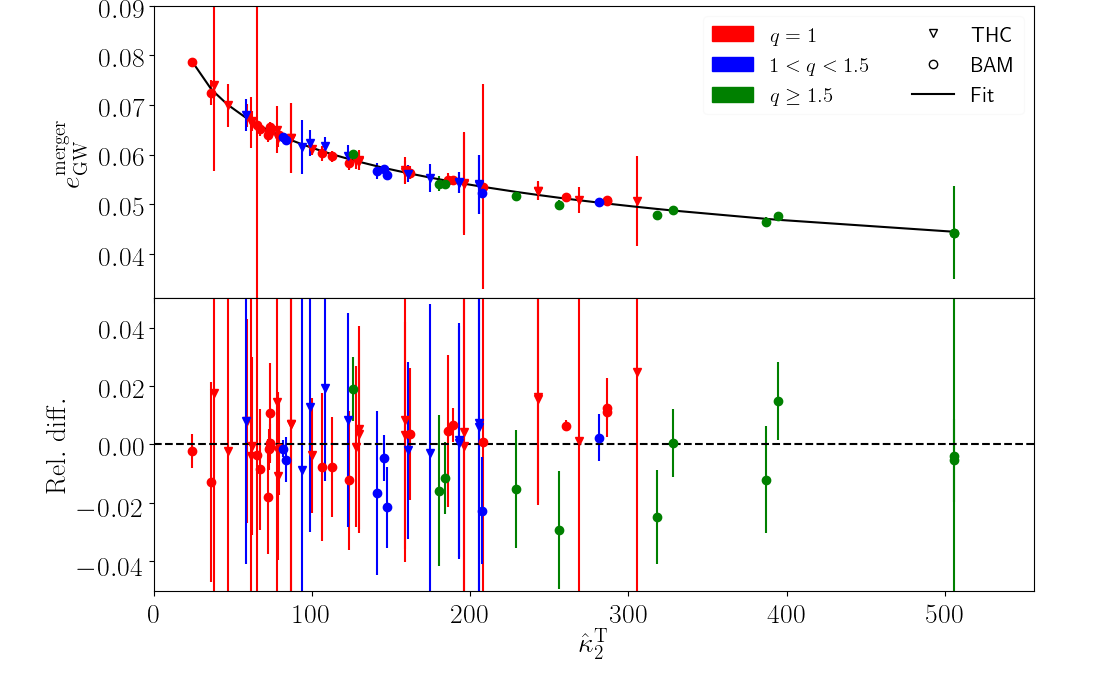
\includegraphics[width=0.9\textwidth]{egw_mrg_fit.png}
  \caption{Fit of the energy per unit mass radiated up to merger.}
  \label{fig:emrg_fit}
\end{figure}

\begin{figure}[t]
  \centering 
  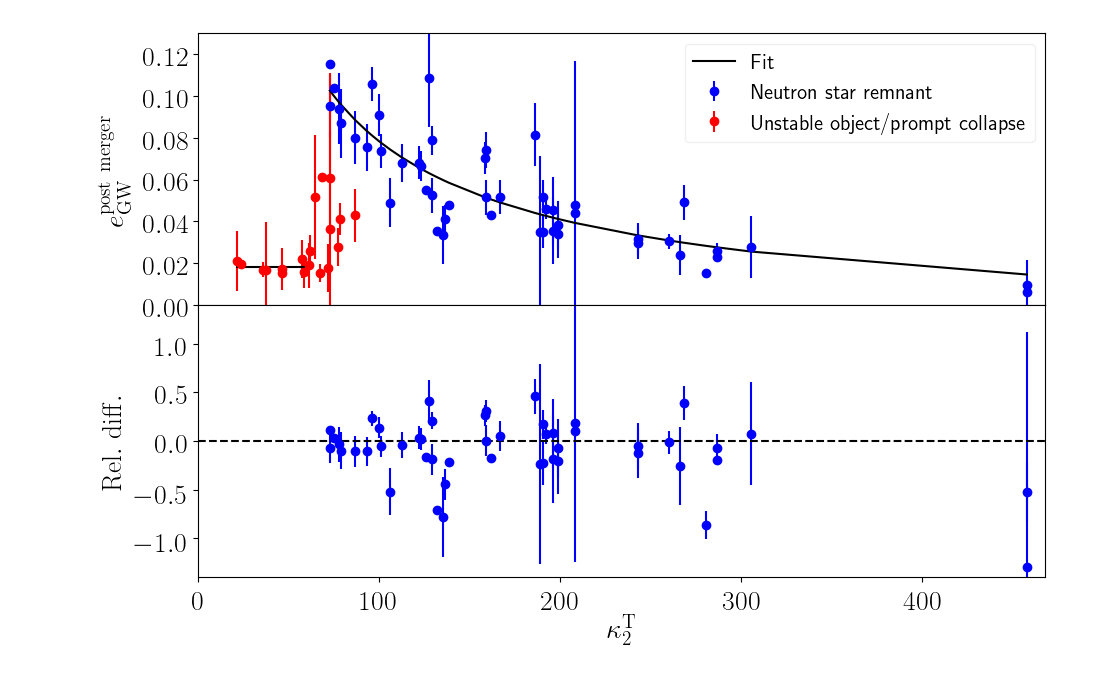
\includegraphics[width=0.9\textwidth]{egw_pm_fitpowerlaw.png}
  \caption{Fit of the energy per unit mass radiated in the post-merger phase.}
  \label{fig:etot_fit}
\end{figure}

%\bibliography{references}

\begin{thebibliography}{1}

%\cite{Zappa:2017xba}
\bibitem{Zappa:2017xba} 
  F.~Zappa, S.~Bernuzzi, D.~Radice, A.~Perego and T.~Dietrich,
  %``Gravitational-wave luminosity of binary neutron stars mergers,''
  Phys.\ Rev.\ Lett.\  {\bf 120}, no. 11, 111101 (2018)
  doi:10.1103/PhysRevLett.120.111101
  [arXiv:1712.04267 [gr-qc]].
  %%CITATION = doi:10.1103/PhysRevLett.120.111101;%%
  %9 citations counted in INSPIRE as of 20 Sep 2018

%\cite{Damour:2009wj}
\bibitem{Damour:2009wj} 
  T.~Damour and A.~Nagar,
  %``Effective One Body description of tidal effects in inspiralling compact binaries,''
  Phys.\ Rev.\ D {\bf 81}, 084016 (2010)
  doi:10.1103/PhysRevD.81.084016
  [arXiv:0911.5041 [gr-qc]].
  %%CITATION = doi:10.1103/PhysRevD.81.084016;%%
  %105 citations counted in INSPIRE as of 20 Sep 2018

%\cite{Dietrich:2018phi}
\bibitem{Dietrich:2018phi} 
  T.~Dietrich {\it et al.},
  %``CoRe database of binary neutron star merger waveforms and its application in waveform development,''
  arXiv:1806.01625 [gr-qc].
  %%CITATION = ARXIV:1806.01625;%%
  %4 citations counted in INSPIRE as of 20 Sep 2018

%\cite{Damour:2011fu}
\bibitem{Damour:2011fu} 
  T.~Damour, A.~Nagar, D.~Pollney and C.~Reisswig,
  %``Energy versus Angular Momentum in Black Hole Binaries,''
  Phys.\ Rev.\ Lett.\  {\bf 108}, 131101 (2012)
  doi:10.1103/PhysRevLett.108.131101
  [arXiv:1110.2938 [gr-qc]].
  %%CITATION = doi:10.1103/PhysRevLett.108.131101;%%
  %48 citations counted in INSPIRE as of 20 Sep 2018

%\cite{Bernuzzi:2015opx}
\bibitem{Bernuzzi:2015opx} 
  S.~Bernuzzi, D.~Radice, C.~D.~Ott, L.~F.~Roberts, P.~Moesta and F.~Galeazzi,
  %``How loud are neutron star mergers?,''
  Phys.\ Rev.\ D {\bf 94}, no. 2, 024023 (2016)
  doi:10.1103/PhysRevD.94.024023
  [arXiv:1512.06397 [gr-qc]].
  %%CITATION = doi:10.1103/PhysRevD.94.024023;%%
  %29 citations counted in INSPIRE as of 20 Sep 2018

%\cite{Keitel:2016krm}
\bibitem{Keitel:2016krm} 
  D.~Keitel {\it et al.},
  %``The most powerful astrophysical events: Gravitational-wave peak luminosity of binary black holes as predicted by numerical relativity,''
  Phys.\ Rev.\ D {\bf 96}, no. 2, 024006 (2017)
  doi:10.1103/PhysRevD.96.024006
  [arXiv:1612.09566 [gr-qc]].
  %%CITATION = doi:10.1103/PhysRevD.96.024006;%%
  %12 citations counted in INSPIRE as of 13 Dec 2018

%% %\cite{Jimenez-Forteza:2016oae}
%% \bibitem{Jimenez-Forteza:2016oae} 
%%   X.~Jiménez-Forteza, D.~Keitel, S.~Husa, M.~Hannam, S.~Khan and M.~Pürrer,
%%   %``Hierarchical data-driven approach to fitting numerical relativity data for nonprecessing binary black holes with an application to final spin and radiated energy,''
%%   Phys.\ Rev.\ D {\bf 95}, no. 6, 064024 (2017)
%%   doi:10.1103/PhysRevD.95.064024
%%   [arXiv:1611.00332 [gr-qc]].
%%   %%CITATION = doi:10.1103/PhysRevD.95.064024;%%
%%   %23 citations counted in INSPIRE as of 20 Sep 2018

%\cite{Bernuzzi:2014kca}
\bibitem{Bernuzzi:2014kca} 
  S.~Bernuzzi, A.~Nagar, S.~Balmelli, T.~Dietrich and M.~Ujevic,
  %``Quasiuniversal properties of neutron star mergers,''
  Phys.\ Rev.\ Lett.\  {\bf 112}, 201101 (2014)
  doi:10.1103/PhysRevLett.112.201101
  [arXiv:1402.6244 [gr-qc]].
  %%CITATION = doi:10.1103/PhysRevLett.112.201101;%%
  %55 citations counted in INSPIRE as of 20 Sep 2018

\end{thebibliography}


\end{document}
